% !TeX spellcheck = en_US
% !TeX root = ../Tom_Sandmann-master_thesis
\section{Interface with the board} \label{sec: Interface with the board}
To interface with the Spartan FPGAs that are present on the SAKURA-G, we make use of Python code from the ChipWhisperer project%
\footnote{\url{https://newae.com/tools/chipwhisperer/}}.
In addition, we make use of the source files for both the main and control FPGAs available on the SAKURA-G website%
\footnote{\url{http://satoh.cs.uec.ac.jp/SAKURA/hardware/SAKURA-G.html}}.
The software needed to develop and deploy hardware designs to our board is as follows:
%
\begin{itemize}
	\item Xilinx ISE 14.7 (licensed);
	\item FTDI drivers D2XX%
	\footnote{\url{http://www.ftdichip.com/Drivers/D2XX.htm}};
	\item FT PROG%
	\footnote{\url{http://www.ftdichip.com/Support/Utilities.htm\#FT_PROG}}.
\end{itemize}
%
The FTDI drivers are required by the \texttt{ftd2xx} Python package to send and receive data to and from one of the FPGAs (i.e. either the control or the main FPGA).
\mintinline{text}{FT_PROG} can be used to view connected FPGAs (if any).
Finally, Xilinx ISE is used to generate the corresponding program files for our design and send them to the board. 

We now describe the structure of the interfaces used in the designs of the control and main FPGAs.
The two FPGAs on the SAKURA-G board are interconnected through a local bus.
The SAKURA-G makes use of an USB FTDI interface that allows an external PC to communicate with the one of the FPGAs.
Channel A of the the USB interface (FT2232H) is connected to the controller FPGA and channel B is connected to the main FPGA.
Depending on the DIP switch (and another control flag), we are connected to either the main FPGA or to the control FPGA.
As we do not need to directly interface with the main FPGA, we assume to be always connected to the USB interface of the control FPGA.

The control FPGA can send and receive data to the main FPGA by making use of the local bus.
The control FPGA also receives external inputs such as a 48MHz clock and a reset signal.
In addition, it can also control the LEDs that are located next to the FPGA on the board.
The 48MHz clock that is received as input by the control FPGA is used to generate two clocks:
one that is used as the system clock (\texttt{clk}), and another one (\mintinline{text}{usb_clk}) to clock the USB connection (which by default is clocked at 24MHz).
The system clock is used in both the local bus (connecting the two FPGAs) and in the main FPGA.
The frequency at which the system clock operates is controlled by the (4-bit wide) User DIP switch (where the default operation frequency is 1.5MHz).
To make use of a different operation frequency, we set the first bit of the DIP switch to high.
The remaining bits of this switch control the new frequency (3, 6, 12 or 24MHz).
A schematic overview of the connection between the two boards can be seen in \Cref{fig: sakura_g-signal-overview}.
%
\begin{figure}
	\centering
	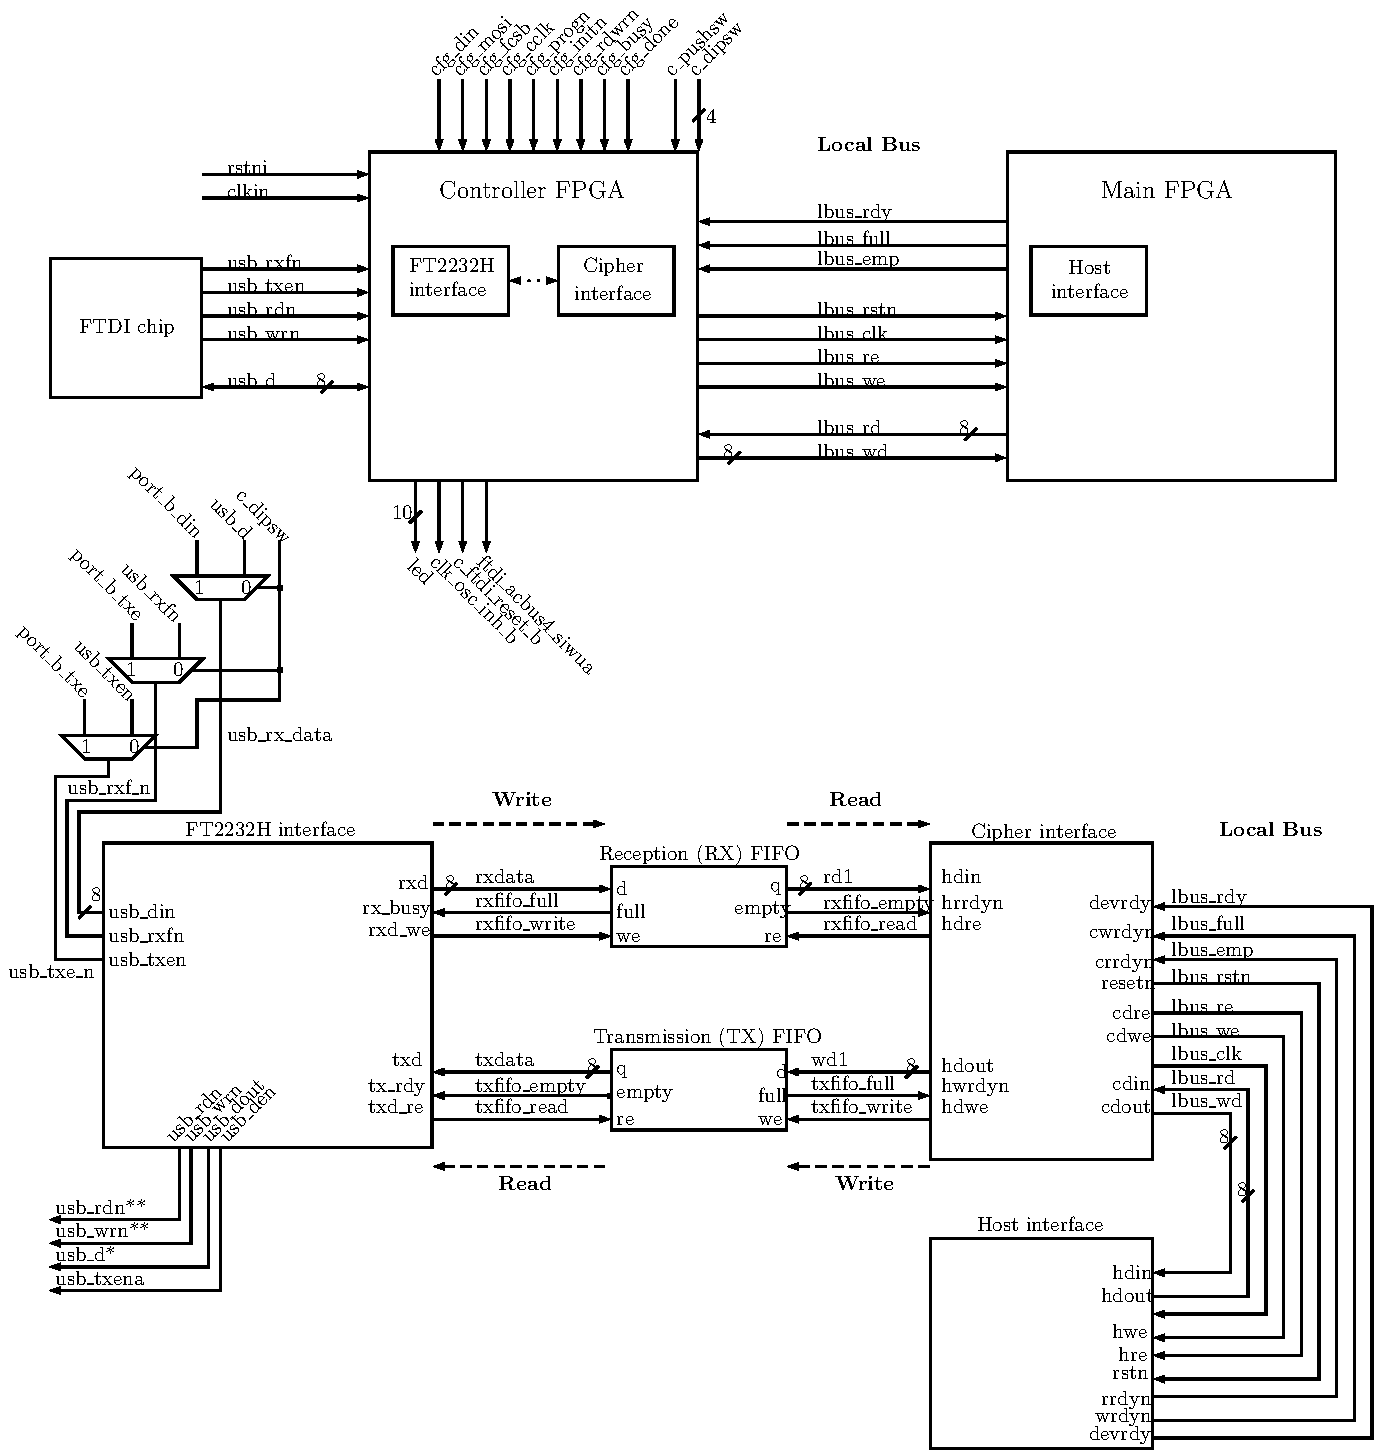
\includegraphics[scale=0.65]{sakura_g-signal-overview}
	\captionof{figure}{Overview of the interfaces used by both the main and control FPGAs. The control FPGA only moves data between the USB port and the control FPGA (via the FT2232H interface) and between the main FPGA and the control FPGA (via the Cipher interface).
	Data transmission between the Cipher interface and the FT2232H interface is done by making use of two FIFOs: a transmission (TX) and a reception (RX) FIFO. 
	The TX FIFO is used to transport data (written by the) Cipher interface to the FT2232H interface,
	while the RX FIFO is used to transport data from the FT2232H interface to the Cipher interface.
	Note that not all input signals are shown (e.g. the clock and reset signals for both FIFOs are omitted).
	The meaning of the single and double stars in some of the output signals from the FT2232H interface are as follows:\\
	%
	\textbf{*}: The value of \mintinline{text}{usb_d} contains the value that is read from the TX FIFO if the first bit of the DIP switch is low (i.e. \mintinline{text}{c_dipsw(0) = '0'})  (and when \mintinline{text}{usb_txena = '1'}). \\
	\textbf{**}: The value of \mintinline{text}{usb_rdn (usb_wrn)} equals the internal \mintinline{text}{usb_rdn (usb_wrn)} signal when the first bit of the DIP switch is low (i.e. \mintinline{text}{c_dipsw(0) = '0'}), otherwise it is a constant value of 1.
	}
	\label{fig: sakura_g-signal-overview}
\end{figure}
%
\begin{figure}
	\centering
	% !TeX spellcheck = en_US

\begin{tikzpicture}[->, >=stealth',shorten >=1pt,auto,node distance=2cm]
\node[state, initial] (idle) {$i$};

\node[state, above right of = idle] (read1) {$r_1$};
\node[state, right of = read1] (read2) {$r_2$};
\node[state, right of = read2] (read3) {$r_3$};

\node[state, below right of = read3] (back off) {$b$};

\node[state, below right of = idle] (write1) {$w_1$};
\node[state, right of = write1] (write2) {$w_2$};
\node[state, right of = write2] (write3) {$w_3$};

\draw (idle) edge[bend left, above] node[align=left, xshift=-40pt]{\mintinline{text}{usb_rxf_reg = '1'} \\ \mintinline{text}{rx_busy = '0'}} (read1);

\draw (idle) edge[bend right, below] node[align=left, xshift=-40pt, yshift=-10]{\mintinline{text}{usb_txe_reg = '1'} \\ \mintinline{text}{tx_rdy = '0'}} (write1);

\draw (read1) edge node{} (read2);
\draw (read2) edge node{} (read3);
\draw (read3) edge[bend left, below] node{} (back off);

\draw (back off) edge node{} (idle);

\draw (write1) edge node{} (write2);
\draw (write2) edge node{} (write3);
\draw (write3) edge[bend right, below] node{} (back off);

\draw (idle) edge [loop above, left, in=-30, out=30, looseness=5] (idle);
\end{tikzpicture}

	\captionof{figure}{Finite state machine used by the FT2232H interface to control the reading and writing from the FTDI USB chip. In the read states ($r_1, r_2, r_3$), a single byte is received from the USB channel in order to be sent to the main FPGA. In the write states ($w_1, w_2, w_3$), a single byte is transmitted over the USB channel.}
	\label{fig: usb_fsm}
\end{figure}
%
We give a short description for each of the interfaces:
%
\begin{itemize}
	\item \textbf{FT2232H interface}: this component reads data from the USB port (FTDI based) and writes in the internal reception FIFO (RX). 
	In addition, it also reads the transmission FIFO (TX) and sends it to the USB port (\Cref{fig: sakura_g-signal-overview}).
	Reading and writing from the FTDI chip is controlled by a finite state machine (FSM) (\Cref{fig: usb_fsm}).  
	This FSM starts in the idle state $(i)$, in which it is determined whether it can start to read data from the USB channel ($r_1$), write data to the USB channel ($w_1$) or remain in the idle state $(i)$. 
	We describe the read and write states in more detail:
	%
	\begin{itemize}
		\item \textbf{Read}. 
		If the RX FIFO is ready and not busy (\mintinline{text}{usb_rxf_reg = '1'} and \mintinline{text}{rx_busy = '0'} respectively), we proceed to the first read state ($r_1$). 
		Once we are in the second read state $(r_2)$, we read the actual byte from the USB channel, and set the write enable of the RX FIFO and indicate that this register is read ready. 
		Finally we proceed to the final read state $(r_3)$, in which the data read from the USB channel is actually written into the RX FIFO. 
		After resetting the write enable of the RX FIFO, we proceed to the back-off state $(b)$.
		
		\item \textbf{Write}.
		If the TX FIFO is ready (\mintinline{text}{usb_txe_reg = '1'} and \mintinline{text}{tx_rdy = '1'}), we proceed to the first write state $(w_1)$.
		In the first write state $(w_1)$, we reset the read enable of the TX FIFO and enable the output of the USB data bus. 
		In the second write state $(w_2)$, we indicate that the value from the TX FIFO is ready to be written to the USB port. 
		
		\item \textbf{Back off}.
		In the back off state $(b)$, we reset the USB write enable (which is low active).
		This signal is passed to the FTDI chip, which then knows that it can set the corresponding signals to send another byte.
		In addition, we also reset the output-enable signal (which indicates whether the output data is valid or not).
		
	\end{itemize}
	%
	\item \textbf{Cipher interface}: This is the interface with the main FPGA. This component controls the local bus between the control and the main FPGA.
	It reads the reception FIFO (RX) that the FT2232H interface writes, and writes content received from the local bus (i.e. written by the host interface) into the transmission (TX) FIFO (see \Cref{fig: sakura_g-signal-overview}).
	Reading and writing from the main FPGA (i.e. the host interface) is controlled by two state machines: 
	%
	\begin{figure}
		\centering
		\subfloat[Finite state machine used by the cipher interface to control the reading from the data written on the local bus by the host interface (i.e. main FPGA).]{
			% !TeX spellcheck = en_US

\begin{tikzpicture}[->, >=stealth',shorten >=1pt,auto,node distance=3cm]
\node[state, initial] (idle) {$i$};

\node[state, right of = idle] (read) {$r$};

\draw (idle) edge[bend left, above] node[align=left]{\mintinline{text}{devrdy = '1'} \\ \mintinline{text}{hwrrdyn = '0'} \\ \mintinline{text}{crrdyn = '0'}} (read);

\draw (idle) edge [loop above, left, out=-60, in=-120, looseness=5] (idle);

\draw (read) edge [bend left, below] (idle);

\end{tikzpicture}

			\label{subfig: cipher read fsm}
		}
		\hspace{0.5cm}
		\subfloat[Finite state machine used by the cipher interface to control the writing to the local bus connected to the main FPGA.]{
			% !TeX spellcheck = en_US

\begin{tikzpicture}[->, >=stealth',shorten >=1pt,auto,node distance=3cm]
\node[state, initial] (idle) {$i$};

\node[state, right of = idle] (fifo read) {$r$};

\node[state, right of = fifo read] (lbus write) {$w$};

%\draw (idle) edge[bend left, above] node[align=left]{\mintinline{text}{hwrdyn = '0'} \\ \mintinline{text}{crrdyn = '0'}} (read);

\draw (idle) edge [loop above, left, out=-60, in=-120, looseness=5] (idle);
\draw (idle) edge node[align=left, yshift = 15] {\mintinline{text}{hwrdyn = '0'} \\ \mintinline{text}{crrdyn = '0'}} (fifo read);
\draw (fifo read) edge (lbus write);
\draw (lbus write) edge[loop above, left, out=120, in=60, looseness=5] node[xshift=30, yshift=10] {\mintinline{text}{cwrdyn = '1'}} (lbus write);
\draw (lbus write) edge [bend left, below] node[align=left]{\mintinline{text}{cwrdyn = '0'}} (idle);

\end{tikzpicture}

			\label{subfig: cipher write fsm}
		}			
		\captionof{figure}{State machines used by the cipher interface to control the reading from and writing to the host Interface.}
		\label{fig: cipher_rw_fsm}
	\end{figure}
	%
	\begin{itemize}
		\item \textbf{Cipher Read} (\Cref{subfig: cipher read fsm}): This state machine controls the reading from data that is written on the local bus by the host interface. The FSM starts in the idle state ($i$), in which it waits until the main FPGA is ready, the host interface is write ready and the cipher interface is read ready (see \Cref{subfig: cipher read fsm}). If this is the case, the FSM moves to the read state $(r)$. In addition, it sets the read enable and clears the write enable of the host. In the read state, the input received over the local bus (\mintinline{text}{lbus_rd}) is written to the TX FIFO. The values of the cipher read and host write enable are restored to their original values.		
			
		\item \textbf{Cipher Write} (\Cref{subfig: cipher write fsm}): This state machine controls the writing on the local bus, which is read by the host interface. The FSM starts in the idle state $(i)$, in which it waits until the host interface is write ready, and the cipher interface is read ready. If this is the case, the FSM moves to a read state in which it reads data from the Reception (RX) FIFO. In the write state, this data is then transmitted over the local bus such that it can be read by the host interface.
	\end{itemize}
	%
	\item \textbf{Host interface}: This component reads and writes the local bus between the control and the main FPGA. It is mainly a state machine. It controls the implementation through the values that are written in the bus. 
	Received values are stored in registers.
	Depending on the received value and the appropriated control signals (e.g. write enable (WE)), parts of the register are assigned specific values.
	This component consists of two registers: \mintinline{shell}{addr_reg} and \mintinline{shell}{data_reg}. 
\end{itemize}
%